\chapter{The Compact Muon Solenoid Experiment}
\label{chap:I-3-cms}

	The Compact Muon Solenoid (CMS) \cite{1748-0221-3-08-S08004} is a multi-purpose particle detector recording the collisions provided by the LHC. It was, along with ATLAS, the first experiment officially approved for the LHC by the CERN research board in January 1997 after a long evalution process of the letter of intent published four years earlier by the collaboration. The construction of the detector started in 2005, after the excavation works of the cavern finished, and spanned until 2008. Since then, CMS has been proficiently taking and analyzing data, and announced on July 4th 2012 the discovery of the Brout-Englert-Higgs boson, one of the most significant results of the collaboraton.

  \section{Overview}

    At nominal energy and luminosity, the LHC produces around 20 proton-proton collisions per BX which results in around 1000 particles in the final state. In order to distingish physical processes with great precission CMS has to ensure good identification and reconstruction of the particles. To this end, the detector was built around four requirements:
    \begin{itemize}
      \item Good muon identification and momentum resolution over a wide range of momenta and angles, good dimuon mass resolution ($ \approx $ 1\% at 100 GeV), and the ability to determine unambiguously the charge of muons with p < 1 TeV;
      \item Good charged-particle momentum resolution and reconstruction efficiency in the inner tracker. Efficient triggering and offline tagging of $ \tau $'s and b-jets, requiring pixel detectors close to the interaction region;
      \item Good electromagnetic energy resolution, good diphoton and dielectron mass resolution ($ \approx $ 1\% at 100 GeV), wide geometric coverage, $ \pi^0 $ rejection, and efficient photon and lepton isolation at high luminosities;
      \item Good missing-transverse-energy and dijet-mass resolution, requiring hadron calorimeters with a large hermetic geometric coverage and with fine lateral segmentation. \\
    \end{itemize}

    \begin{figure}[h!]
      \centering
      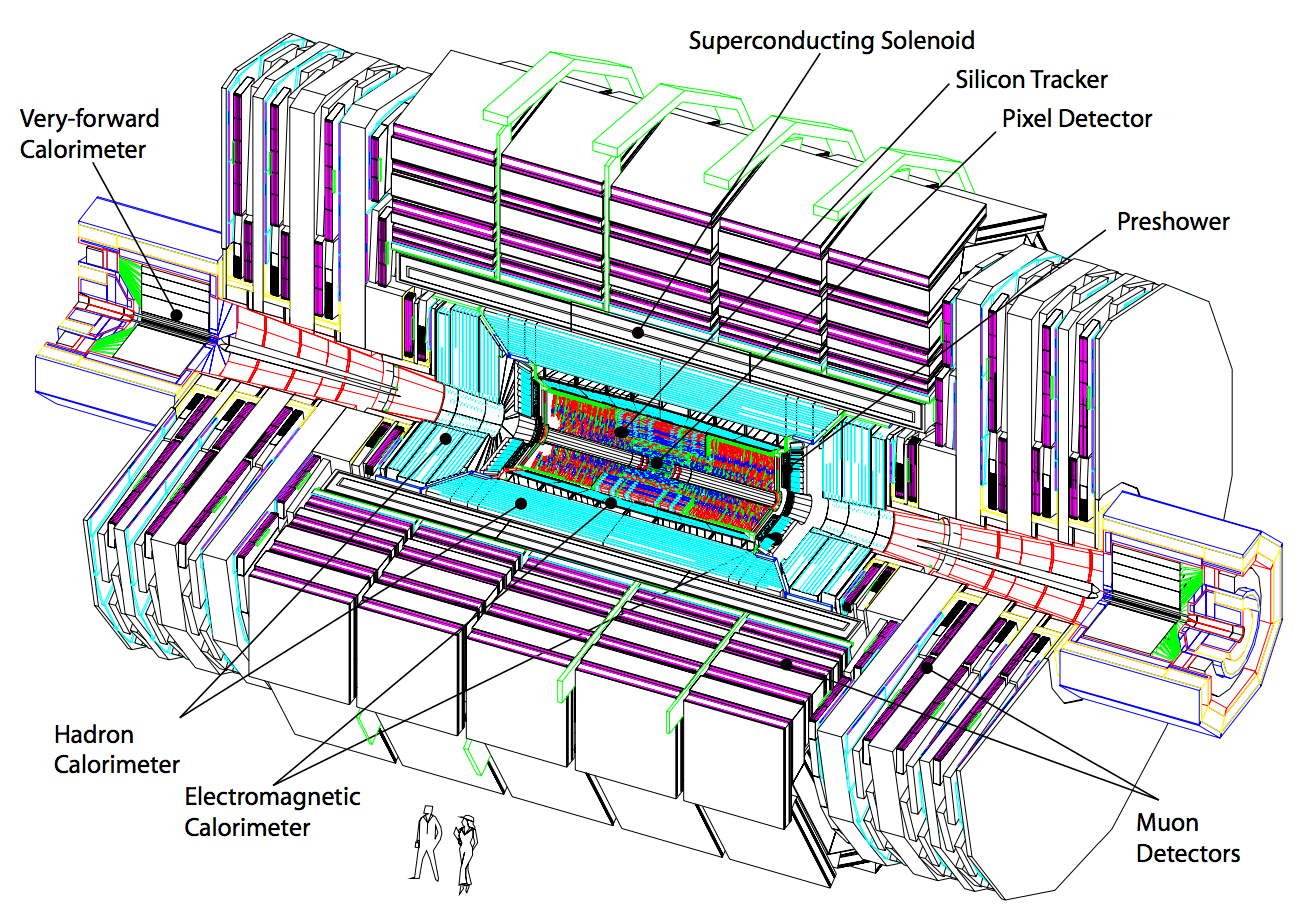
\includegraphics[width=\textwidth]{img/I-3-cms/cms.png}
      \caption{Schematic representation of the Compact Muon Solenoid detector installed at LHC \cite{1748-0221-3-08-S08004}.}
      \label{fig:I-3-cms-global-view}
    \end{figure}

    These requirements are met through the subdivision of CMS in various detection systems each specialised in the reconstruction of a given type of particles. The overall layout of CMS, shown in Figure \ref{fig:I-3-cms-global-view}, is divided into the barrel and the two endcaps, regions where the detectors are respectivly placed in parrallel and perpendicularly to the beam pipe. At the center of the detector, closest to the interaction point, lies the inner tracking system. Composed of 3 layers of silicon pixels and 10 layers of silicon strips detectors, it is designed to detect the passage of any charged particle with high precision. Surrounding the tracking system are the electromagnetic and hadronic calorimeters which respectivly measure the energy of electrons and photons, and hadrons. These detectors are placed inside a superconducting solenoid magnet which produces a strong 3.8 T field that bends charged particles and allows for precise momentum measurments. Outside of the magnet, three different technologies of muon detectors are placed on large iron yokes. Furthest from the interaction point are the very-forward calorimeters which intercept particles with low flighing angle.

    The coordinate system used in CMS has its origin at the nominal interaction point of the beams, the y-axis pointing upwards, the x-axis pointing toward the center of the LHC, and the z-axis directed along the beam direction. The polar coordinates (r, $ \phi $) are defined in the x-y transverse plane and the widely used pseudorapidity $ \eta $ is taken to be
    \begin{equation}
      \eta = - \ln\left( \tan\left( \frac{\theta}{2} \right) \right) ,
    \end{equation}
    where $ \theta $ is the azimuthal angle between the z-axis and the transverse plane.

  \section{The Inner Tracking System}

    The inner tracking system of CMS is designed to provide a precise and efficient hit information on the trajectories of charged particles.  The proximity of the detectors to the beam pipe yields a high particle density of up to 10$^8$ particles per cm$^2$ at a radius of 4 cm. This justifies the need for a high granularity and fast response time to unambigously assign particles to the correct collision. However, these features come with an elevated power comsumption which in turn requires efficient cooling infrastructure. In order to keep the material budget of the tracker as low as possible, a compromise was found to use two technologies: silicon pixels close to the beam pipe to provide a high granularatiy, and silicon strips further away to reduce the material budget. \\

    The layout of the detectors is shown in Figure \ref{fig:I-3-tracker}. The silicon pixels (PIXELS) are installed on three cylindrical layers in the barrel and two disks in each endcap. These detectors cover an area between radii of 4.4 cm and 10.2 cm and a pseudorapidity $|\eta|$ > 2.5. The silicon strips (TIB, TOB, TEC, and TID) occupy a radial region between 20 cm and 116 cm and are divided in different sectors with a total of 10 layers in the barrel and 12 disks in each endcap. The segmentation into sectors corresponds to the various strip geometries and arrangment. \\

    \begin{figure}[h!]
      \centering
      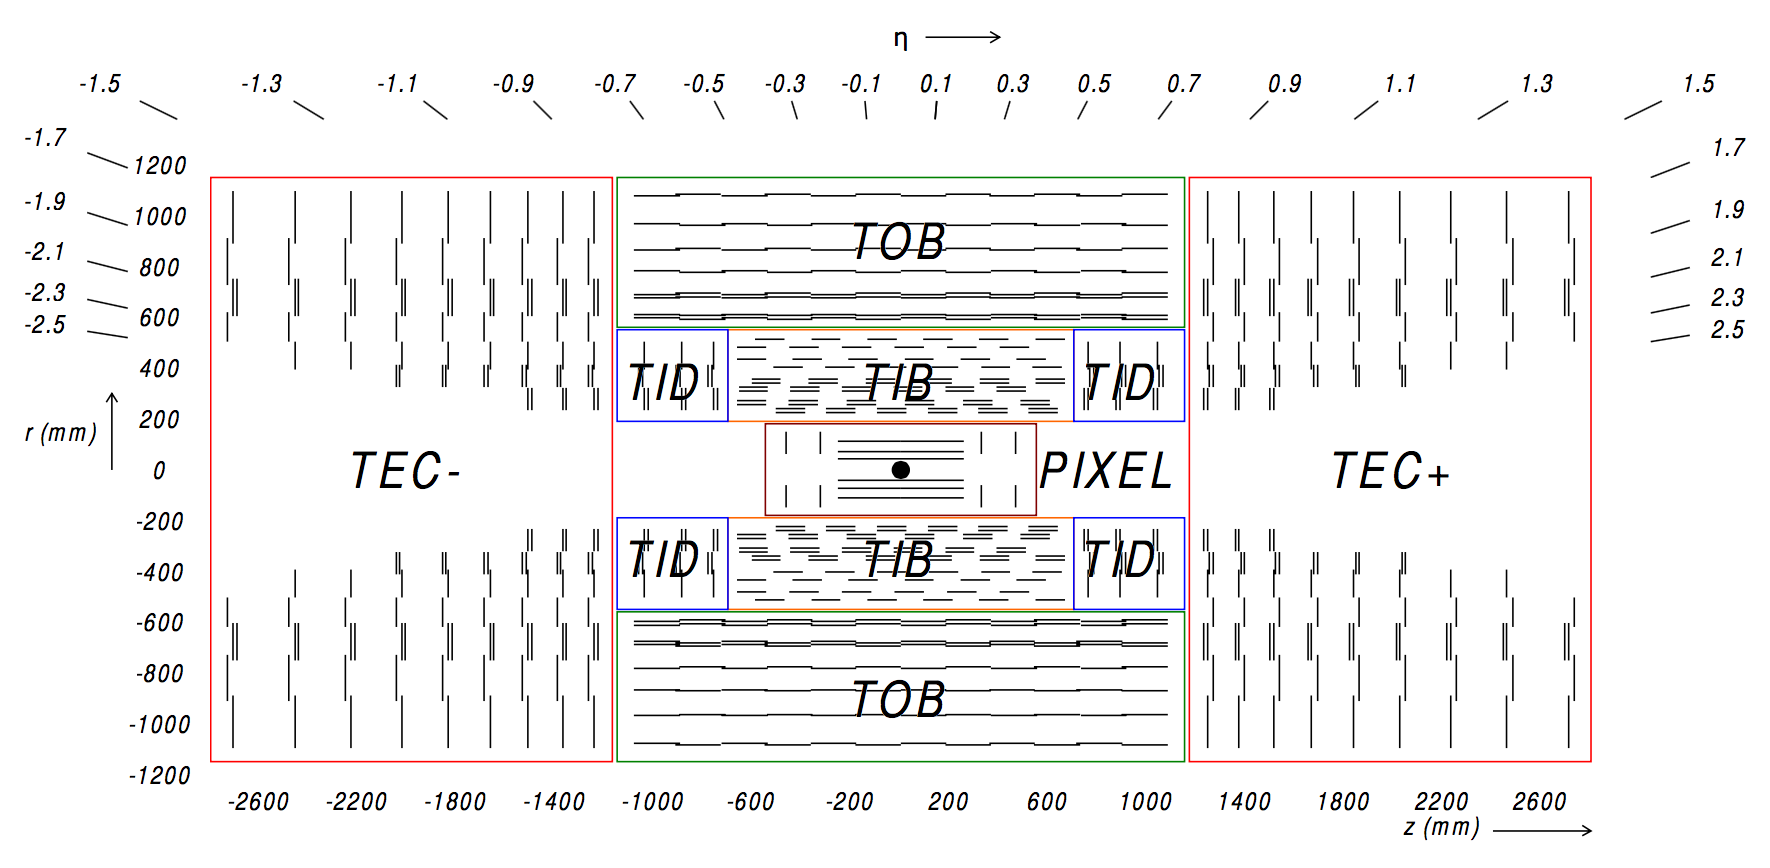
\includegraphics[width=\textwidth]{img/I-3-cms/tracker.png}
      \caption{Schematic representation of the Compact Muon Solenoid detector installed at LHC \cite{1748-0221-3-08-S08004}.}
      \label{fig:I-3-tracker}
    \end{figure}

    The barrel pixel tracker contains 768 modules for a total of 48 million pixels. The disks of the endcaps are divided into 24 segments each composed of 7 modules which yields a total number of 672 modules with 18 million pixels for the both endcaps. Each pixel is 150 $\mu$m $\times$ 100 $\mu$m in size with a thickness of 260 $\mu$m to 300 $\mu$m resulting in a single point hit resolution of 15 $\mu$m to 20 $\mu$m. \\

    The silicon strip tracker is divided into three subsystems. The Tracker Inner Barrel and Disks (TIB/TID) are composed of 4 layers in the barrel and 3 disks in each endcap, covering a region up to 55 cm. The strips are 320 $\mu$m thick and run parallel to the beam pipe in the barrel and radially in the disks. The strip pitch is of 80 $\mu$m in the two first layers of the TIB and 120 $\mu$m in the two next ones, resulting in a spatial resolution of respectivly 23 $\mu$m and 35 $\mu$m. In the TID, the pitch varies between 100 $\mu$m and 141 $\mu$m. Surroungind the TIB and TID is the Tracker Outer Barrel (TOB) composed of 6 barrel layers of 500 $\mu$m thick strips. It provides a resolution of 53 $\mu$m for the first four layers and 35 $\mu$m for the two last ones. Closing the TOB on both sides are the Tracker EndCaps (TEC) which each hold 9 disks. In addition, given modules are equipped with a second strip detector mounted back-to-back with a stereo angle of 100 mrad to provide a measurment of the second coordinate.

  \section{The Electromagnetic Calorimeter}

    The Electromagnetic Calorimeter (ECAL) of CMS is composed of lead tungstene (PbWO$_4$) crystals that act as hermetic calorimeters: they initiate the particle cascades and providing the proportionnal response to the energy deposition. The barrel counts 61 200 crystals closed by 7 324 crystals in each endcap. In order to distinguish pion shower, a high granularity preshower is installed in front of the ECAL, providing detailed measurments of the impact points. \\

    The structure of the ECAL is shown in Figure \ref{fig:I-3-ecal}. In the barrel, the ECAL covers a pseudorapidity range $ | \eta | $ < 1.479 and is divided in 360 sections in $ \phi $ and 170 in $ \eta $. The crystals cross-section varies between 22 mm $ \times $ 22 mm to 26 mm $ \times $ 26 mm for a length of 230 mm corresponding to 25.8 radiation lengths. In the endcaps, the modules cover a pseudorapidity 1.479 < $ | \eta | $ < 3.0. Each crystal has a front cross-section of 28.62 mm $ \times $ 28.62 mm and a length of 220 mm. They are grouped in units of 5 $ \times $ 5 crystals called supercrystals further inserted in one of the two \emph{Dees} that compose an endcap and maintains the ECAL in place. The preshower uses a lead radiators to initiate the avalanche that will be detected by silicon strips to measure the deposited energy and the avalanche profile. \\

    \begin{figure}[h!]
      \centering
      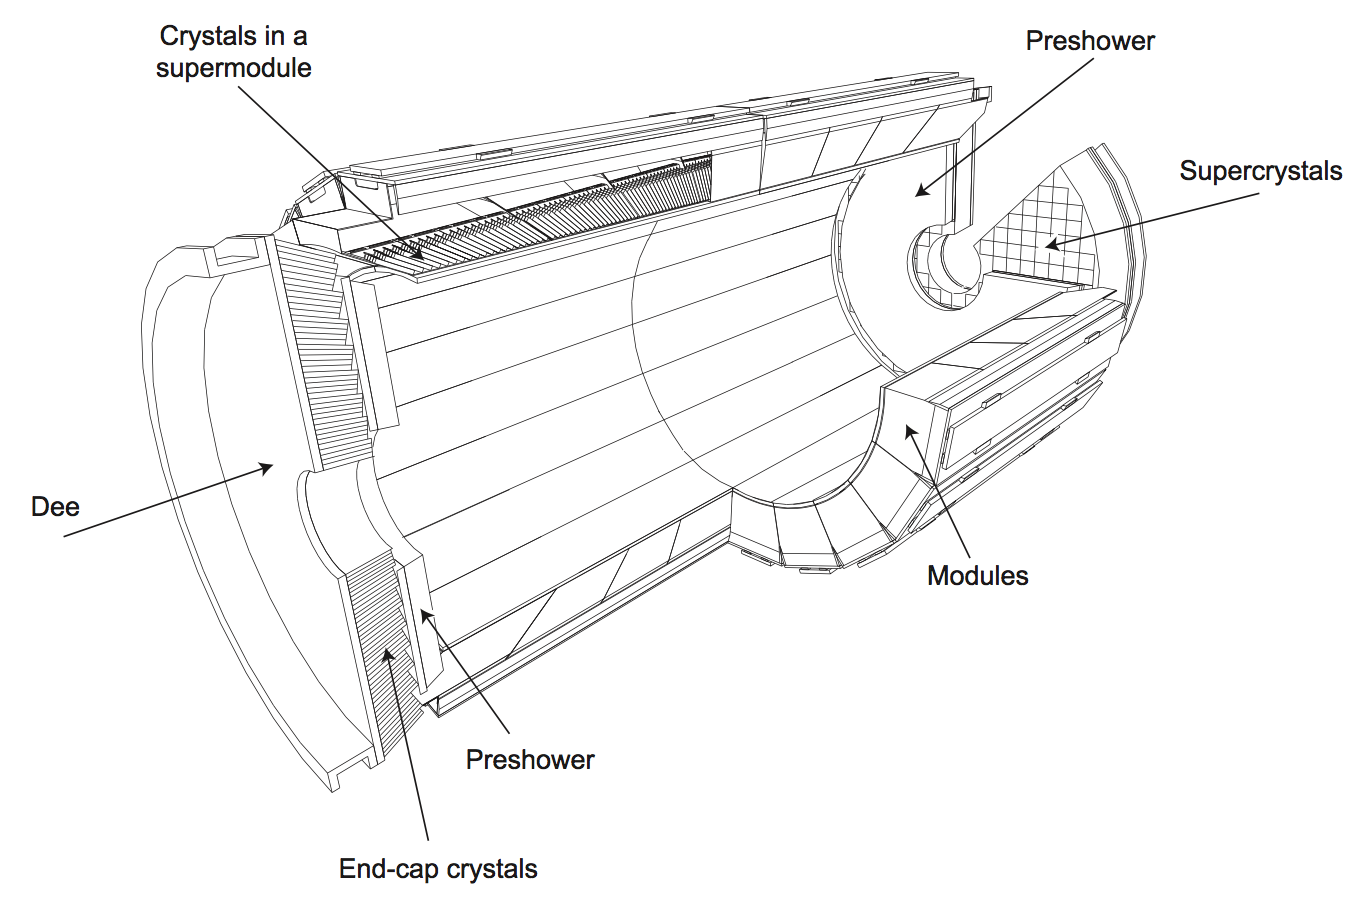
\includegraphics[width=\textwidth]{img/I-3-cms/ecal.png}
      \caption{Layout of the ECAL and disposition of the crystals in modules and supermodules \cite{1748-0221-3-08-S08004}.}
      \label{fig:I-3-ecal}
    \end{figure}

    The energy resolution of the ECAL for particles with energy bellow 500 GeV is parametrized by the following equation:
    \begin{equation}
      \left( \frac{\sigma}{E} \right)^2 = \left( \frac{S}{\sqrt{E}} \right)^2 + \left( \frac{N}{E} \right)^2 + C^2
    \end{equation}
    where $ S $ is the stochastic term, $ N $ the noise terme, and $ C $ the constant term. The main contributions to the stochastic term are relatated to fluctuations in the lateral shower containment, photostatique contributions, and fluctuations in the energy deposition inside the preshower radiators compared to what is measured by the silicon detector. The noise term includes noise from the electronics, the digitisation, and pile-up. Finally, the constant term accounts for non-uniformities in the crystals, callibration errors, and leakage of energy from the back of the crystals. From test beams, the values of $ S $, $ N $, and $ E $, where found to be so that: \\
    \begin{equation}
      \left( \frac{\sigma}{E} \right)^2 = \left( \frac{2.8\%}{\sqrt{E}} \right)^2 + \left( \frac{0.12}{E} \right)^2 + (0.30\%)^2
    \end{equation}

  \section{The Hadron Calorimeter}

    The Hadron Calorimeter (HCAL) is divided into a barrel region (HB), two endcaps regions (HE), and an outer calorimeter (HO) placed right outside the magnet as represented in Figure \ref{fig:I-3-hcal}. An additionnal forward calorimeter (HF) is place in the very forward region of CMS. The HB sits between the ECAL and the magnet at radii of 1.77 m and 2.95 m respectivly which limits the amout of material and thus absorption lengths that can be used, justifying the need for the HO to catch the trail of the cascades. \\

    \begin{figure}[h!]
      \centering
      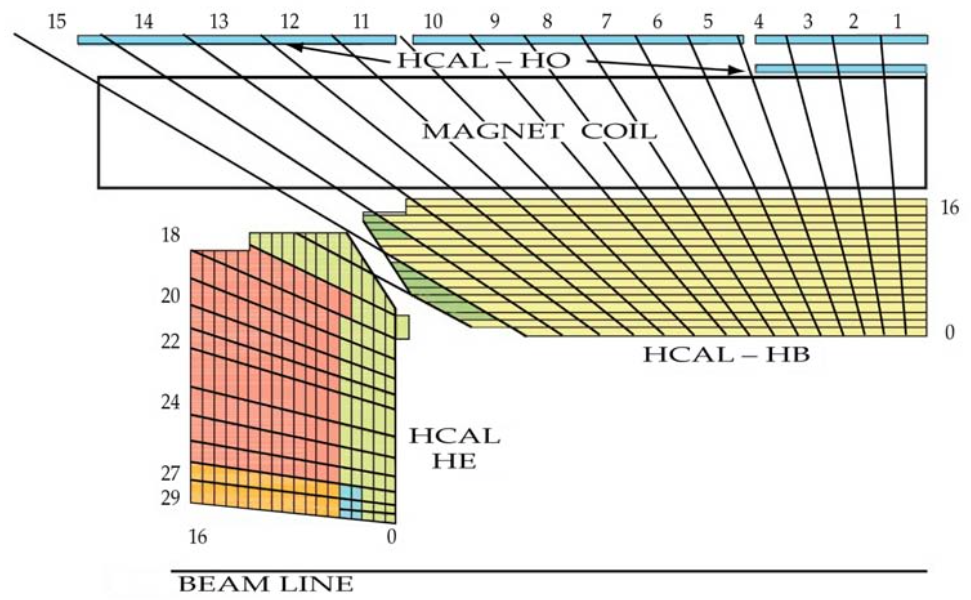
\includegraphics[width=\textwidth]{img/I-3-cms/hcal.png}
      \caption{Layout of the HCAL and disposition of the crystals in modules and supermodules \cite{1748-0221-3-08-S08004}.}
      \label{fig:I-3-hcal}
    \end{figure}

    The HB uses a sampling calorimeter design that consists of a succession of metal sheets positonned parallel to the beam that act as absorber and plastic scintillators to measure the energy deposition. The absorber is made of a 40 mm thick front steel panel, followed by eight 50.5 mm thick brass sheets, six 56.5 mm thick brass panels, and a 75 mm thick steel back plate for a total minimum of 5.82 interaction lengths. The scintillators are designed out of 3.7 mm thick Kuraray SCSN81 plastic and placed after each layer of metal. An additionnal layer of 9 mm thick Bicron BC408 is placed in front of the first steel panel in order to sample hadronic showers that might have formed in the ECAL. The HE uses 79 mm thick brass plates spaced by 9 mm gaps in which the plastic Bicron BC408 scintillators are inserted. The segmentation of the HE results in a granularity of $ \Delta \eta \times \Delta \phi $ = 0.087 $ \times $ 0.087 for $ | \eta | $ < 1.6 and 0.17 $ \times $ 0.17 for $ | \eta | $ $ \le $ 1.6. In the $ | \eta | $ < 1.3 region, hadron showers are not entierly contained in the HB and HE thus justifying the installation of the HO outside of the magnet to catch the trail of the cascades. This has a significant impact on high energy cascades and to measure the missing energy of an event, i.e. the energy carried by non-interracting particles. The HO has a minimum thickness of 1.4 interaction lengths and is segmented in 5 rings further divided into segments. Each segment has a granularity similar to the HB of 0.087 $ \times $ 0.087 in $ \Delta \eta \times \Delta \phi $. Limited by the muon system, the HO has been allocated 40 mm of space, from which 16 mm is used for the scintillators and the rest is filled with support material.

  \section{The Superconducting Magnet}

    The superconducting magnet of CMS measures 6 m of diameter for 12.5 m in length and has been design to generate a 4 T magnetic field. The return of the magnetic field lines is done through the steel yokes that support the muon chambres of CMS as represented in Figure  \ref{fig:I-3-cms-magnet} in which the amplitude of the magnetic field inside CMS has been measured using cosmic muons. The magnet is composed of four layers of winded NbTi conductor which offers very low resistance to the nominal 19.14 kA current that is required. To reach the superconducting state of the magnet, it needs to be cooled down to 1.8 K. The magnetic field thereby created bends charged particles according to their transverse momentum in the x-y plane
    \begin{equation}
      R = \frac{p_T}{0.3 B} ,
    \end{equation}
    where $ R $ is the curvature radius of the trajectory in the transverse plane, $ p_T $ is the transverse momentum of the particle expressed in GeV, and $ B $ is the intensity of the magnetic field in T.

    \begin{figure}[h!]
      \centering
      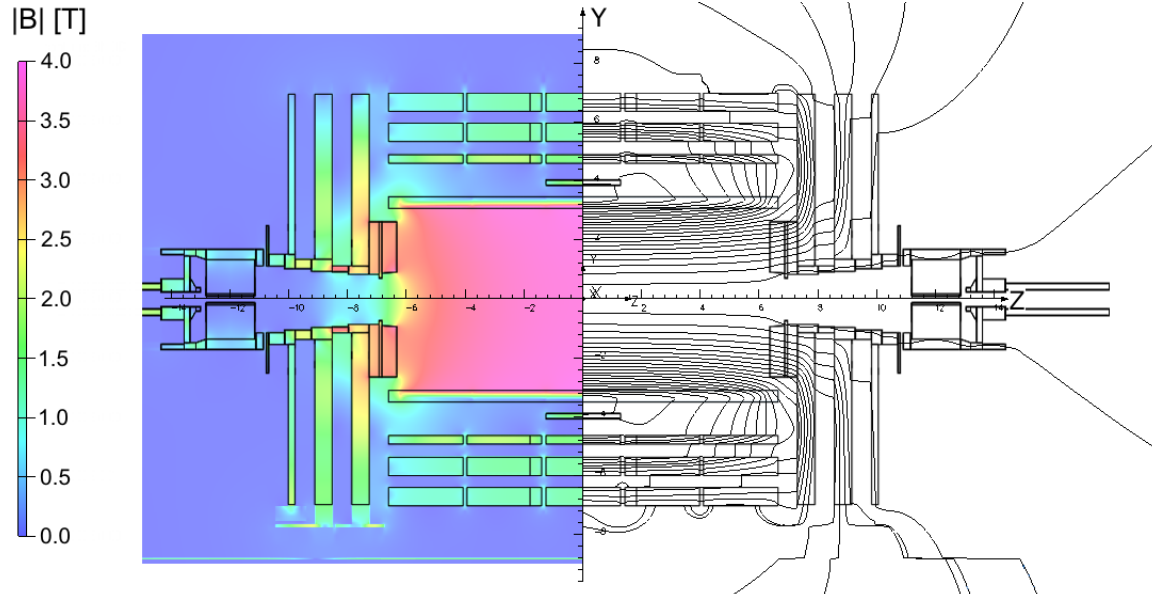
\includegraphics[width=\textwidth]{img/I-3-cms/magnet.png}
      \caption{??? \cite{Chatrchyan:2009si}.}
      \label{fig:I-3-cms-magnet}
    \end{figure}

  \section{The Muon System}

    Muons are a recognizable signature from the high background noise produced by the high number of p-p interactions. Moreover, they are present in many processes that characterize interesting processes from the standard model and beyond. Therefore, providing good triggering, identification, and reconstruction capabilities is essential. CMS is equipped with three different muon detectors that together form the muon spectrometer: Drift Tubes (DTs), Cathode Strip Chambers (CSCs), and Resistive Plate Chambers (RPCs). DTs and CSCs are respectivly placed in the barrel and the endcaps while RPCs are installed in both regions, adding redunduncy to the system by providing additionnal measurment points. Figure \ref{fig:I-3-muons} represent a quadrant of CMS highlighting the placement of the various technologies inside the detector. \\

    In the barrel, four cylindrical layers of DTs, numbered MB1 to MB4, are spread over a pseudorapidity range of $ | \eta | $ < 1.2. The first three layers each contain modules of eight chambers: four to measure the r-$\phi$ bending angle and four to measure the z direction. The fourth station solely tracks the r-$\phi$ parameter using four chambers. \\

    In the endcaps, the CSCs cover a region of 0.9 < $ | \eta | $ < 2.4 and are spread over four disks where detectors are placed perpendicularly to the beam pipe. Each disk is further divided into two or three rings number MEx/y, where x is the disk number and y is the ring number. CSCs measure both the r-$\phi$ and the $ \eta $ parameter using respectivly cathode strips that run radially and anode wires that run perpendicular to the strips. Each module is composed of 6 layers of CSCs which provide precise background noise rejection and tracking. \\

    In order to provide fast triggering and improve the time resolution, RPCs, which provide a fast timing response, are installed in front of the DTs and CSCs label RBx and REx/y. In the barrel, two stations of RPCs are installed in RB1 and RB2 while only one station is instrumented in RB3 and RB4. In the endcaps, one module of RPCs equips each of the stations except for the first ring of each disk which has been left empty. This is due to the high rate of particles in the region close to the beam pipe which is not supported by the RPCs.

    \begin{figure}[h!]
      \centering
      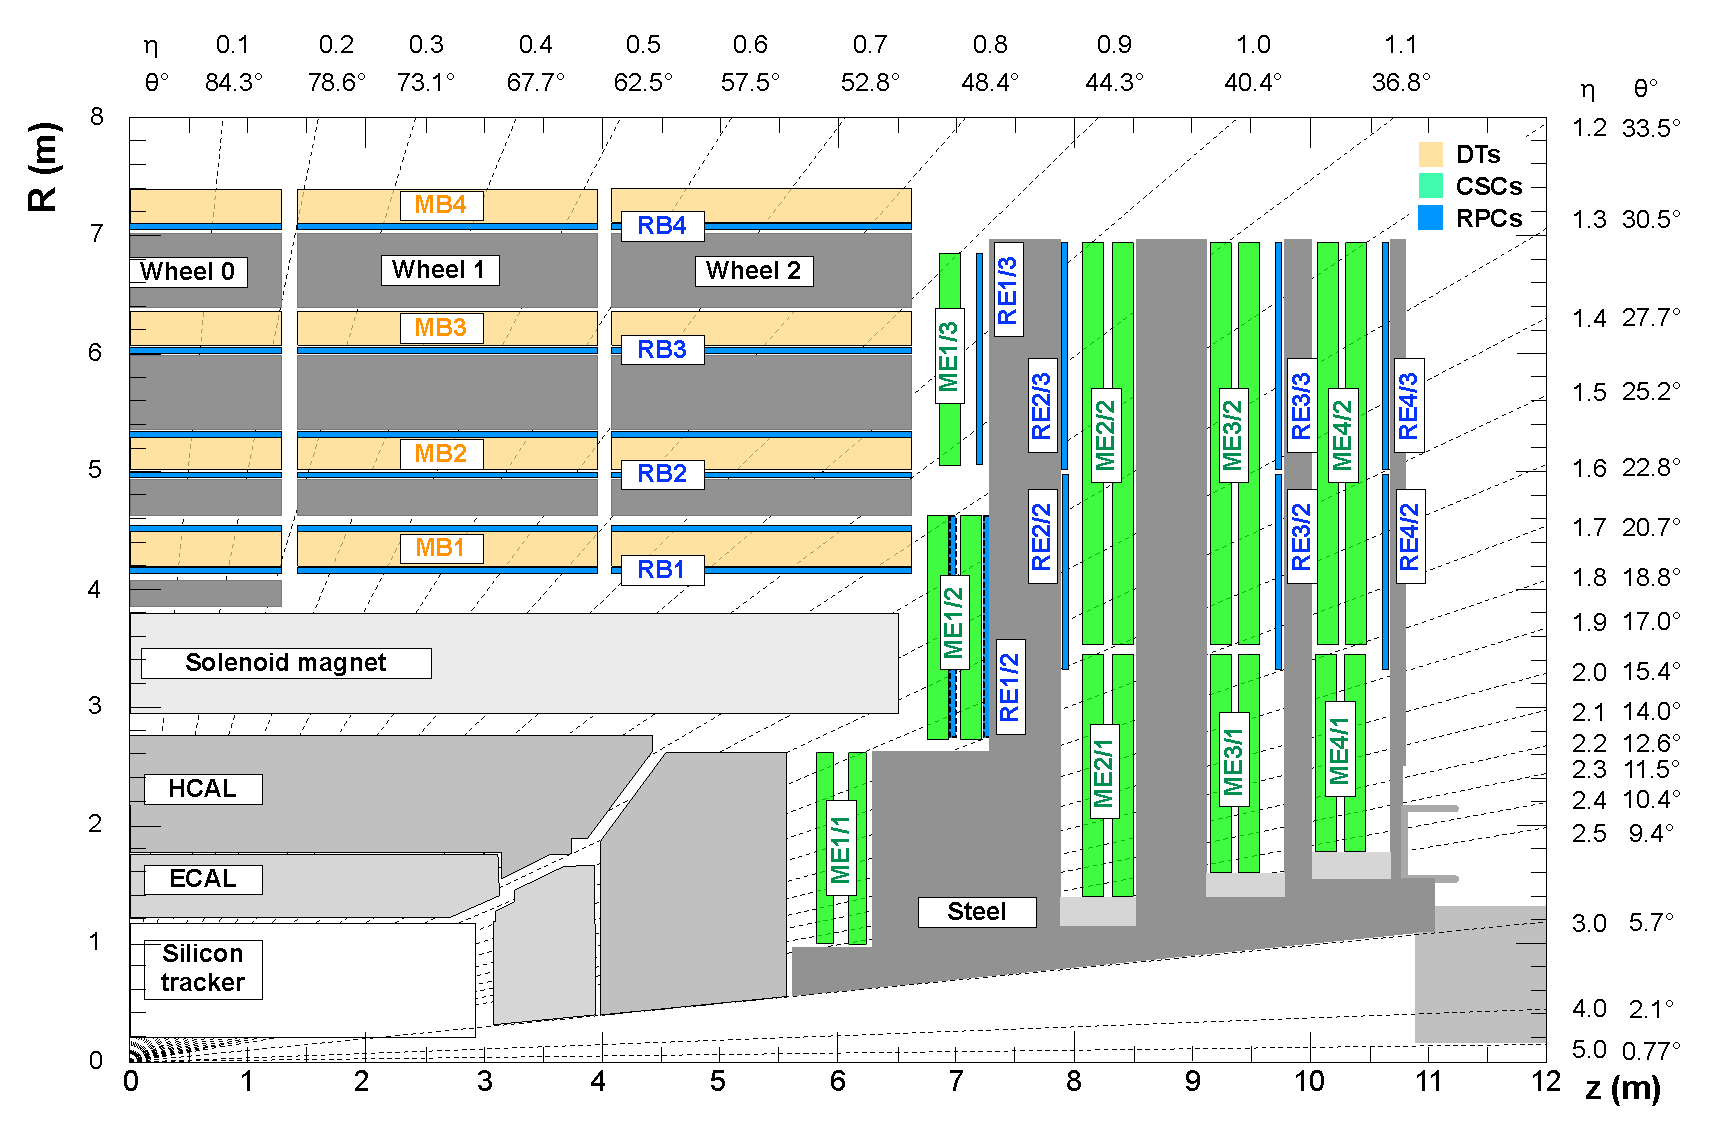
\includegraphics[width=\textwidth]{img/I-3-cms/muons.pdf}
      \caption{??? \cite{1748-0221-3-08-S08004}.}
      \label{fig:I-3-muons}
    \end{figure}

    \subsection{Drift Tubes}

  	\subsection{Cathode Strip Chambers}

  	\subsection{Resistive Plate Chambers}
